%------------------------------------------------------------------------
%  交通流のシミュレーション 
%  The Mathematical Society of Traffic Flow
%  
%  Ver. 1.0 05/12/09  H. Watanabe
%------------------------------------------------------------------------

\documentclass[twocolumn]{jarticle} %二段組の場合
%\documentclass[onecolumn]{jarticle}  %一段組の場合

\usepackage{mstf2}
\usepackage[dvipdfmx]{graphicx}
\usepackage{graphicx}
\usepackage{mathtools}
\graphicspath{{./pic/}}
\usepackage{gensymb}
%------------------------------------------------------------------------

%------------------------------------------------------------------------
%コンパイルコマンド
%1. platex thesis.tex
%2. platex thesis.tex
%3. dvipdfmx thesis.dvi
%4. evince thesis.pdf &
%------------------------------------------------------------------------


\title{%和文タイトル
非線形感覚運動写像ロボットの対面流\\
{\Large -- 1方向走行流への転移と流量のコース幅依存性 --}
}

\titleE{%英文タイトル
Counter flow of robots based on non-linear sensorymotor mapping\\
{\large -- Dependence on the course width of transition to one-direction flow and flow rate --}
}

\author{%和文氏名
李 方正$^1$, 橋爪 晋平$^2$,本田 泰$^3$
}

\authorE{%英文氏名
Li Fangzheng$^1$, Shimpei Hashizume $^2$,Yasushi Honda $^3$
}

\affiliation{%和文所属
$^1$ 室蘭工業大学大学院 工学研究科 情報電子工学系専攻\\
$^2$ 室蘭工業大学 工学部 情報電子工学系学科\\
$^3$ 室蘭工業大学大学院 しくみ解明系領域
}

\affiliationE{%英文所属
$^1$ Division of Information and Electronic 
Engineering, Graduate School of Engineering, Muroran Institute of Technology, Japan\\
$^2$ Department Information and Electronic 
Engineering,  School of Engineering, Muroran Institute of Technology, Japan\\
$^3$ College of Information and Systems, Muroran Institute of Technology, Japan
}

\abst{%和文概要

In previous research,we did some pseudo-ellipse course experiments of Face-to-Face movement with seasory motor mapping robots based on tanh function.
Then,we comfirmed the transference phenomenon from Face-to-Face movement to one-direction flow and measure the flow rate and time from start to one-direction flow.

In this paper, in order to shun one-direction flow, we made neural network model(input:960,middle:1000,output:2) which can analyse one-dimension image data and
did about five experiments of  neural network model and seasory motor mapping model in same course. 
From those experiments we know the robots can avoid obstacles smoothly and keep Face-to-Face movement for a long time successfuly.
Beside, we also proved the neural network model is better than seasory motor mapping model in robots flow rate, time of keep one-direction flow and turn around number through compare between two model.

 


}

\abstE{%英文概要
Counter flow of self-driving particles which include insect herd behavior and 
human walking in crowded situations is a widespread phenomenon.

In this study, we have developed sensorimotor-mapping robot which can avoid 
ocstacles using nonliner function (hyperbolic function) and we regard those 
robots as self-driving particle.

Then we have carried out experiments in which these robots start from a counter flow 
in some oval-course, and we found a transition phenomenon from counter
flow to one-direction flow.
We have measured the flow rate and the transition time to 
one-direction flow. 


}

%------------------------------------------------------------------------
% ここから本文
%------------------------------------------------------------------------

\begin{document}
\maketitle

\section{はじめに}
   実世界で,蜂,アリなどの昆虫が簡単な行動メカニズムによって,複雑な群れ行為ができる.
また,大きな交差点などにおいて,人間は密度が高くても,会話なしで,
ぶつからないようにスムーズに対面歩行ができる.

池田ら\cite{ikeda16}は,非常に密度の高い自己駆動粒子の対面流において異方性を考慮
することによってレーン形成が生成することを見出した.

本論文では,我々は原生生物レベルの反応行動のための知能を持つ走行ロボットを開発した.
コース幅が限られたコースにおける,その走行ロボットの対面走行を実験的に観察する.

今回,最大8台使われるロボットを時計回りと反時計回りの2つグループを分けて
楕円コースでの対面走行を実験を行った.
コース幅を変化させ,ロボットの振舞いを観察した.
ロボットが,1方向走行流になるまでの時間と流量などロボットの基本的な走行情報を測定した.

\section{非線形感覚運動写像ロボット}
\subsection{ロボットの身体性}
   今回使っているのは4輪走行ロボットである,
人間や昆虫の走行特徴に近似するため,その場で曲がり,方向転換が可能である.
距離センサーが赤外線の反射で距離を測るので,超音波より測る範囲が狭いが,
体積が小さく,精度が高くて,複数ロボットの場合,ロボット同士間の妨害も減少できる.
\vspace{-2mm}
\begin{figure}[h]
    %\begin{minipage}{0.48\linewidth}
        \centering
        \includegraphics[width=0.6\linewidth]{robot1.jpg}
        \caption{正面図, A,B,C:右,中央,左の距離センサー;
                 D:カメラ(今回使っていない);
                 E,F:左右のモーター;
                 左右センサー角度:45\degree;
                 ロボット幅:13.5cm;ロボット長さ:20.2cm;ロボット高さ:12.2cm;
        }
    %\end{minipage}
    %\begin{minipage}{0.48\linewidth}
    %    \centering
    %    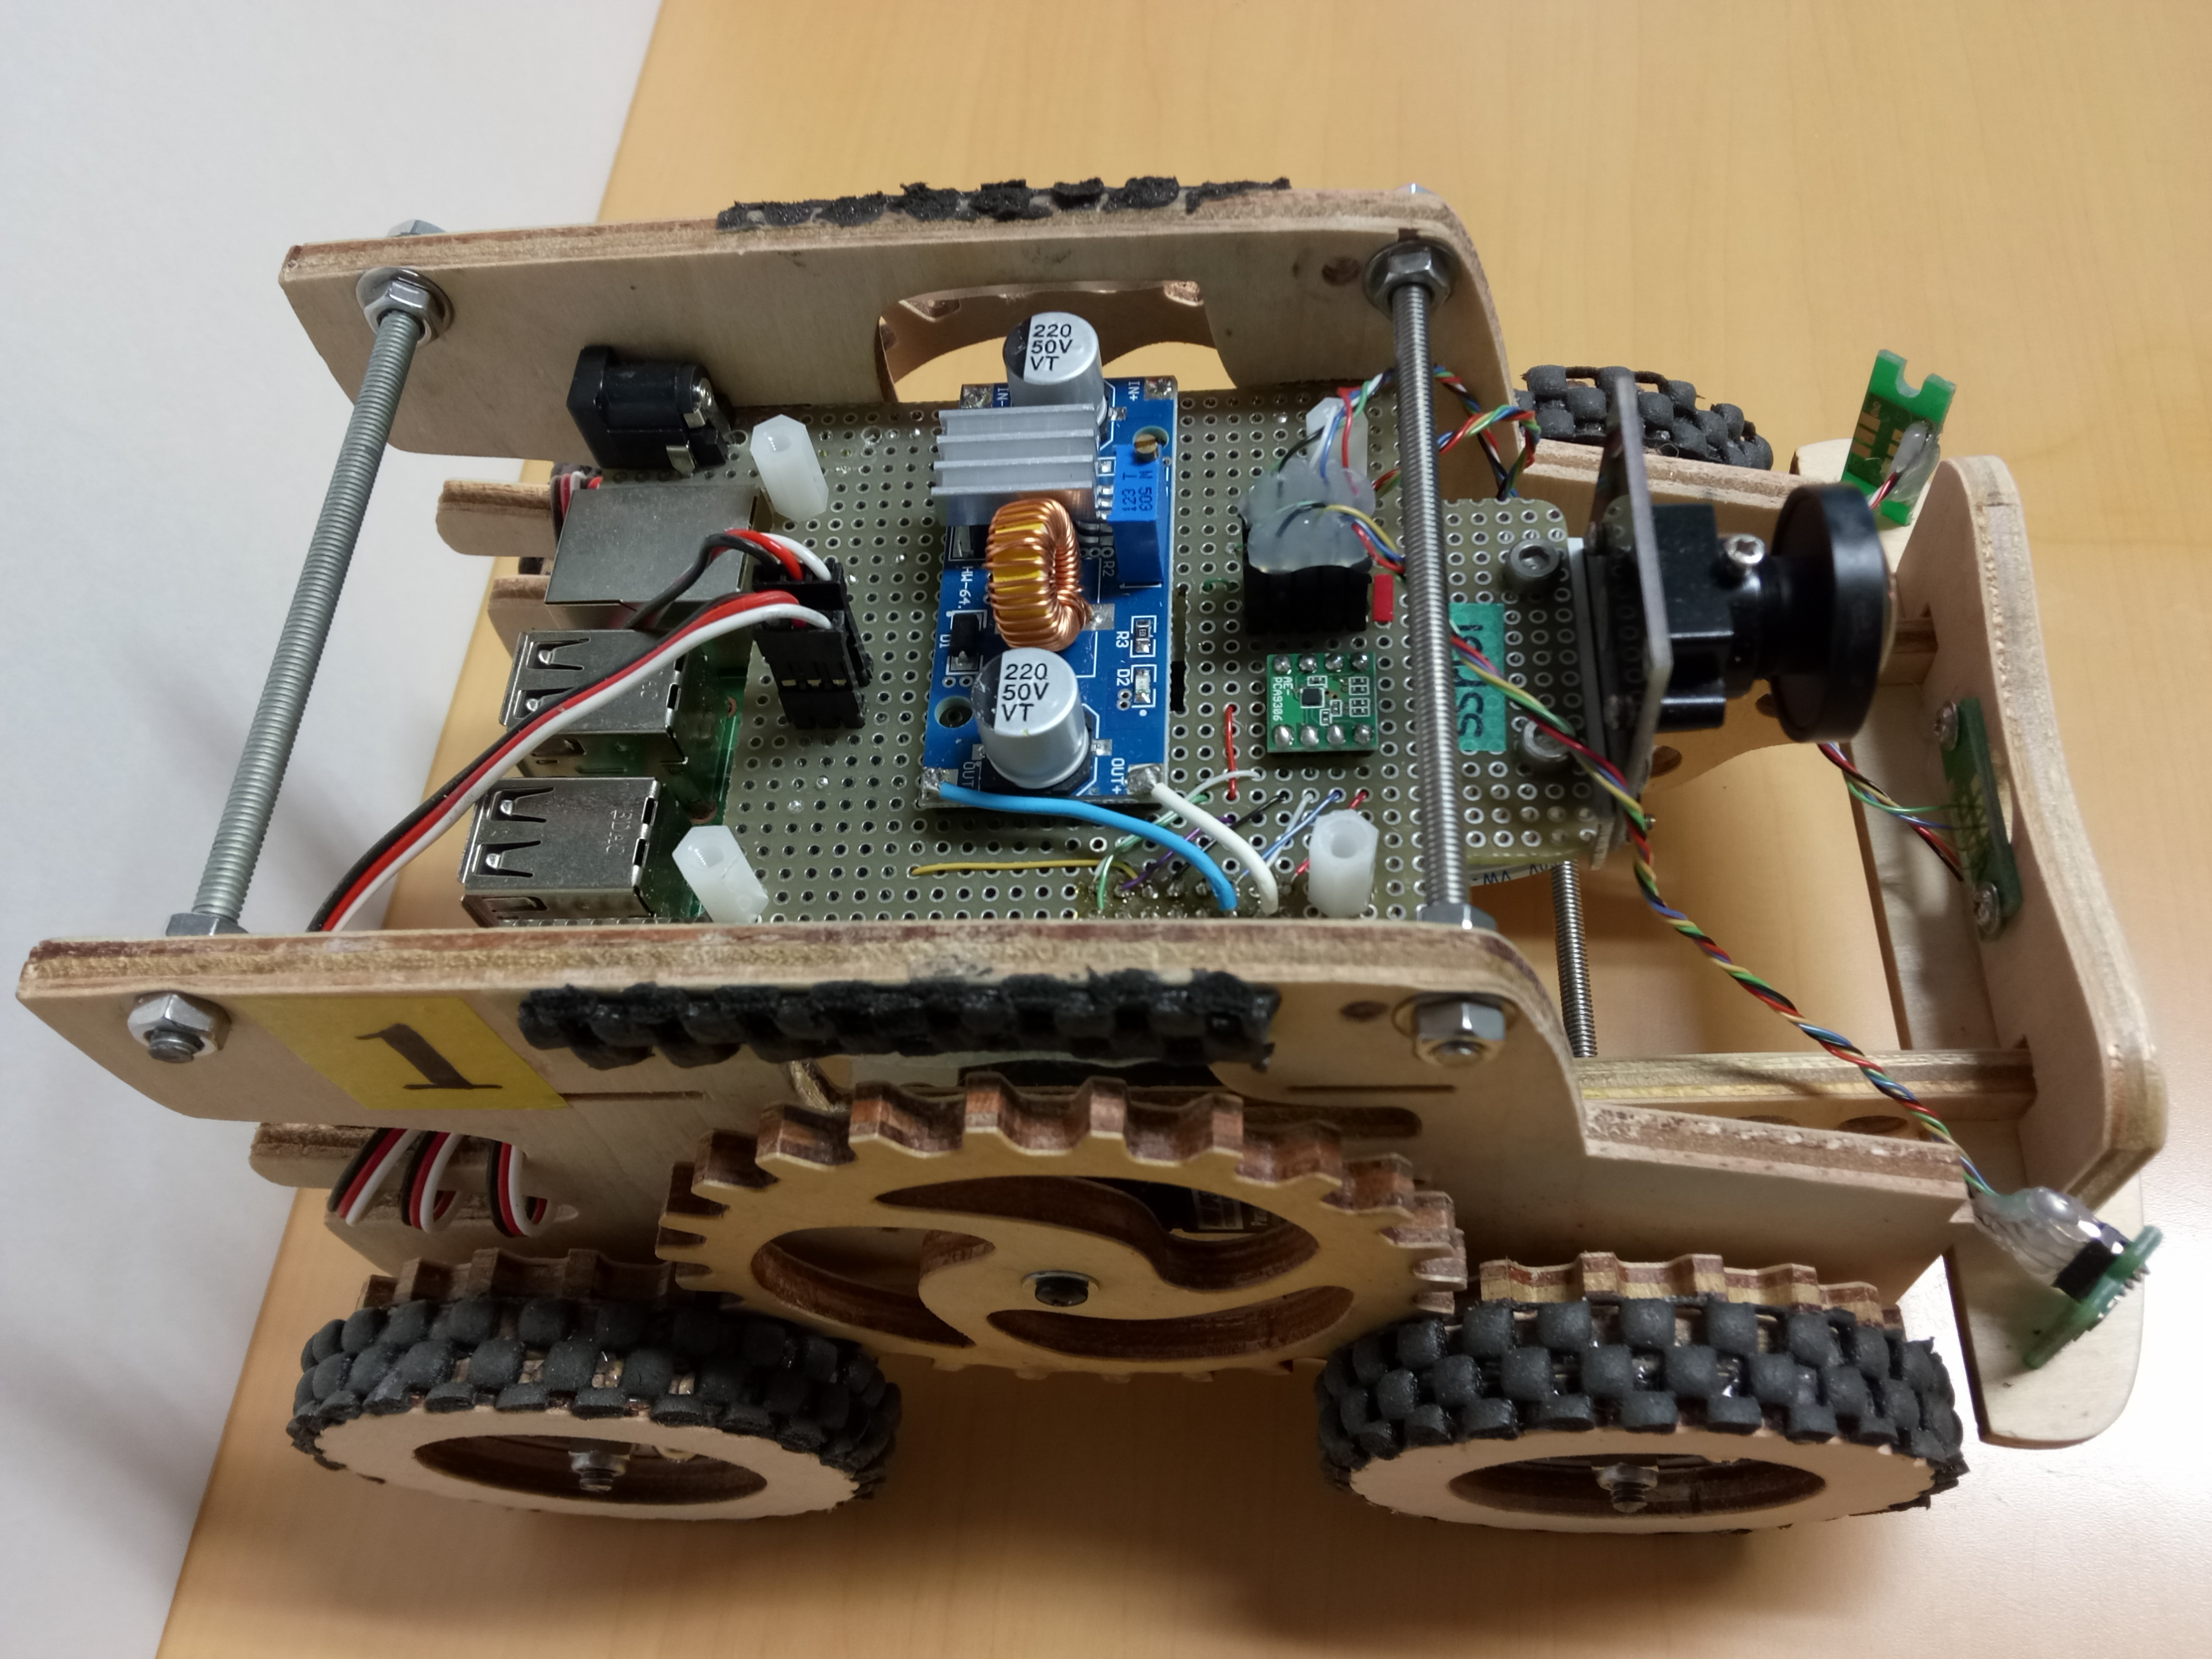
\includegraphics[width=0.9\linewidth]{robot2.jpg}
    %    \caption{俯瞰図}
    %\end{minipage}
\end{figure}
%\vspace{-6mm}
%\begin{figure}[h]
%        \centering
%        \includegraphics[width=1.0\linewidth]{robot4.jpg}
%        \caption{左右のセンサー角度表示}
%\end{figure}




\subsection{ロボット駆動アルゴリズム}
   感覚運動写像とは,センサー値を変数とする関数によってモーターの出力を決定することであり,
その瞬間のセンサー値だけを使う,最も単純な反応行動のための知能の一つである\cite{asada}.
本研究では,非線形感覚運動写像モデルが使われている.

\subsection{距離データの加重相乗平均}
中央のセンサーによる距離データを $d_{\rm C}$,
また,左のセンサーによる距離データを $d_{\rm L}$ とする.
それらを用いて,左の感覚運動写像の入力 $x_{\rm L}$ を加重相乗平均によって
求める(式(\ref{eq:xL})).
同じように,$d_{\rm C}$と右のセンサーから得られた距離データ $d_{\rm R}$を
用て右の感覚運動写像の入力 $x_{\rm R}$ を求める(式(\ref{eq:xR})).
\begin{eqnarray}
  %x_{\rm L} &=& e^{\gamma \ln d_{\rm C}} \cdot e^{(1-\gamma)\ln d_{\rm L}} 
  x_{\rm L} &=& d_{\rm C}^{\gamma} \times d_{\rm L}^{(1-\gamma)}
  \label{eq:xL} \\
  %x_{\rm R} &=& e^{\gamma \ln d_{\rm C}} \cdot e^{(1-\gamma)\ln d_{\rm R}} 
  x_{\rm R} &=& d_{\rm C}^{\gamma} \times d_{\rm R}^{(1-\gamma)}
  \label{eq:xR}
\end{eqnarray}
$\gamma$は重みであり,本研究においては$\gamma=0.33$とする.
$\gamma=\frac{1}{3}$とすることにより,左のセンサー,中央のセンサーおよび右の
センサーがそれぞれ,$\frac{2}{3}$の等加重となる.

\subsection{感覚運動写像}
式(\ref{eq:xL})と式(\ref{eq:xR})で得られた$x_{\rm L}$と$x_{\rm R}$を式(\ref{eq:mR})と
式(\ref{eq:mL})に代入して,ロボットの右モーターの出力($m_{\rm R}$)と左モーターの
出力($m_{\rm L}$)を計算する.
係数$\alpha$がロボットの最大速度を制御する,係数$\beta$が{\rm tanh}の傾きを制御する.
係数$b$が関数の変曲点の位置を制御する,係数$c$が関数の縦軸上の位置を制御する.
\begin{eqnarray}
\begin{aligned}
  m_{\rm R} = &\alpha \tanh(\beta_1(x_{\rm L} - b_{\rm L})) + \\
        &\alpha \tanh(\beta_2(x_{\rm L} - b_{\rm L})) + c
 \label{eq:mR}
\end{aligned}
\end{eqnarray}

\begin{eqnarray}
\begin{aligned}
  m_{\rm L} = &\alpha \tanh(\beta_1(x_{\rm R} - b_{\rm R})) + \\
        &\alpha \tanh(\beta_2(x_{\rm R} - b_{\rm R})) + c
 \label{eq:mL}
\end{aligned}
\end{eqnarray}
 
今回の実験のパラメーターは
$\alpha=30\%$とする.
すなわちロボットは最高速度の60\%の速度で走行する.
$\beta_1=0.004$,
$\beta_2=10$,
$c=0$とする.
ロボットグループ1の$b_{\rm L}$とロボットグループ2の$b_{\rm R}$は160mm,
また,ロボットグループ2の$b_{\rm L}$とロボットグループ1の$b_{\rm R}$は260mmである.

\subsection{パラメーター$b$の説明}
$b_{\rm L}=260$mm(図\ref{fitan}のB点),$b_{\rm R}=160$mm(図\ref{fitan}のA点)の場合,
$b_{\rm L}=260$mmのtanh関数の変曲点が$b_{\rm L}=160$mmのtanh関数の変曲点より横軸の正方向に
100移動して(図\ref{fitan}の$B$点),$x-b_{\rm L}$が小さくなる,式(\ref{eq:mR})により,
右のモーターが左のモーターより先に速度を減少するので,ロボットが右曲がりやすい.
左に曲がり易いのは逆である.
%\vspace{-9mm}
\begin{figure}[!ht]
    \centering
    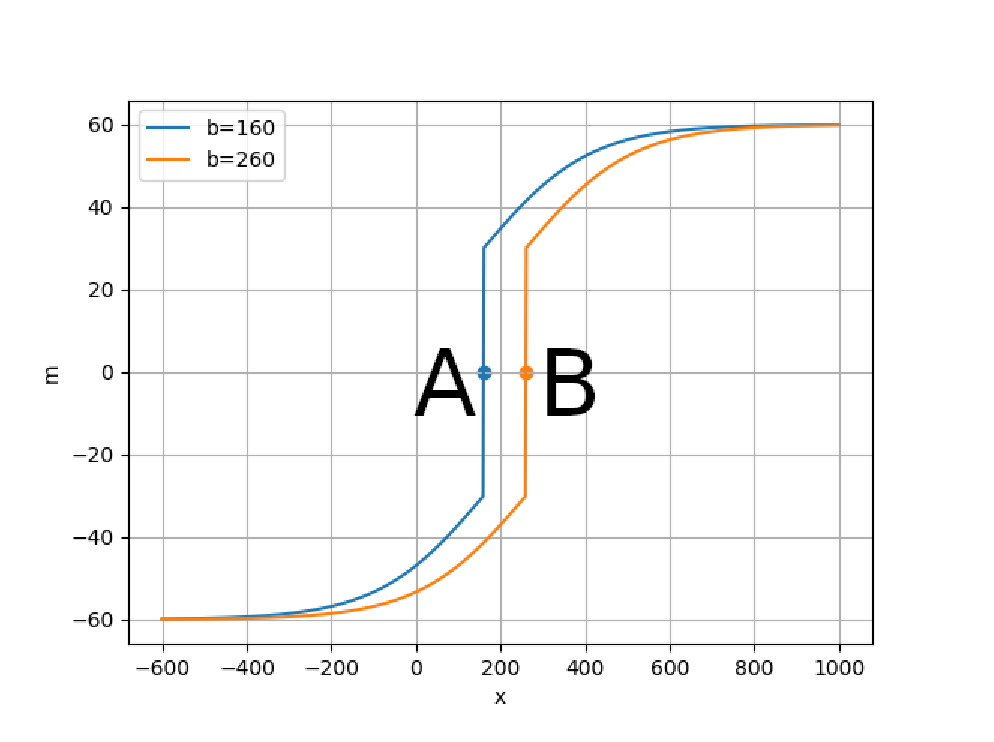
\includegraphics[width=0.7\linewidth]{tanh.eps} 
    \caption{$b=160$mmと$b=260$mmのtanh関数の曲線}
    \label{fitan}
\end{figure}


\section{走行実験}
   本文は内側半径1mの円と外側半径2mの円で作られた幅1mの円形コースで実験する.
内側のコース壁を薄青色に塗って,
外側のコース壁を青色の縞模様としている.
時計回りロボット4台と反時計回りロボット4台を2つずつセットにしてコースの中にランダムに置いて,
約8分間実験した.ロボットが自分の向きを判断できるため,


ロボットが破線1から反時計回りで破線2まで移動して,$\theta$が0から$\pi$に変わる.
破線1から時計回りで破線2まで移動して,$\theta$が0から$-\pi$に変わる.
$R$はロボットからコース中心までの距離である(Fig.\ref{courseshitar}).
それに,ロボットが反時計回りで破線1を通過したら,通過回数$n_{ij}$が+1,
ロボットが時計回りで破線1を通過したら,通過回数$n_{ij}$が-1になる.
次,ロボット一台ずつ,各自の$n_{ij}$を計測して,
各ロボットの通過回数の絶対値を足し算して,1回の実験の通過回数になる.
$T_i$は$i$番目の実験の1方向走行流になる時間です(先行研究\cite{li}の$T_{\rm 1d}$と同じ,単位:min),
$n_{ij}$が$T_i$以内の通過回数です,1方向走行流になた後の通過回数を捨てた.
(\ref{eq:flow})式で$i$番目の実験の流量$Q_i$を求めて,
(\ref{eq:flow_ave})式で流量の平均値を求める.
本研究の流量が対面流の流量である.
$j$はロボットの番号で,
$k$はロボットの台数です(今回の実験で1から8まで合計8台ロボットを使ったので,$k=8$.

$w$がコースの幅(単位:m),
$N_{\rm exp}$は全実験回数を表す.

ロボットが渋滞状態を解消する能力も比較するため,2つロボットをペアとして,
ランダムの初期配置(Fig.\ref{randstart})と渋滞の初期配置(Fig.\ref{crowdstart})の実験を行った

\vspace{-1mm}
\begin{figure}[h]
        \centering
        \includegraphics[width=0.6\linewidth]{shitaR.eps}
        \caption{実験の様子(俯瞰図)と$\theta$の説明}
        \label{courseshitar}
\end{figure}

\vspace{-2mm}
\begin{eqnarray}
Q_i &=& \frac{\sum_{j=1}^{k} |n_{ij}|}{wT_i}
\label{eq:flow} \\
\bar{Q} &=& \frac{1}{N_{\rm exp}}\sum_{i=1}^{N_{\rm exp}} Q_i
\label{eq:flow_ave} 
\end{eqnarray}

\vspace{-1mm}
\begin{figure}[h]
    \begin{minipage}{0.49\linewidth}
        \centering
        \includegraphics[width=1.0\linewidth]{startrand.eps}
        \caption{ランダムの初期配置}
        \label{randstart}
    \end{minipage}
    \begin{minipage}{0.49\linewidth}
        \centering
        \includegraphics[width=1.0\linewidth]{start_crowd.eps}
        \caption{渋滞の初期配置}
        \label{crowdstart}
    \end{minipage}
\end{figure}

\section{実験結果}
\subsection{$T_{\rm 1d}$の測定}
  図\ref{fig:ssr}は8台のロボットの$\theta$(図\ref{course1}参照)と時間の関係図である,
横軸は時間($秒$),縦軸は角度$\theta$(rad)である.

\begin{figure}[!ht]
     \centering
     \includegraphics[width=1.0\linewidth]{ssr4_1.png}
\end{figure}

\vspace{-8mm}
\begin{figure}[!ht]\label{ssr2}
     \centering
     \includegraphics[width=1.0\linewidth]{ssr4_2.png}
     \caption{コース中心から見たロボットの角度$\theta$の時間変化}
     \label{fig:ssr}
\end{figure}


$T_{\rm 1d}$とは全てのロボットが方向転換せず,
同じ向きで走る状態になる時間である,
図\ref{fig:ssr}中の黒い線はロボットが方向転換しなくなるまでの時間,
その中で一番長いものを$T_{\rm 1d}$とする.





\subsection{初期配置}
   ロボットの初期配置はランダムで,グループ1のロボットが左回りの向き,
グループ2のロボットが右回りの向きとする.

%\item $T_{\rm sd}$:全てのロボットのスタートから全てのロボットが一方向走行するまでの所要時間

%各ロボットの平均速度を
%各ロボットが一台で5周回って,$v=\frac{5*L}{t}$で時速を計算する($v$:時速,$L$:コースの長さ,$t$:5周回る時間).時速の平均値$\bar v$:13.125$m/min$;標準偏差($s$):51.384


\subsection{幅による$T_{\rm 1d}$と流量の測定}
   コースの幅が5つあり,それぞれの幅で十回(毎回8分間)実験する,一実験毎に,ランダムにロボットを2つグループを分ける.$T_{\rm 1d}$と流量($Q$)を計測して,平均値と標準偏差を計算する.
%\begin{table}[!ht]
%\setlength\tabcolsep{1pt}
%\begin{center}
%\begin{tabular}{|c|c|c|c|c|}
%\hline
%幅& $\bar{T}_{\rm 1d}$ & $s_{T_{\rm 1d}}$ & $\bar Q$ & $s_Q$ \\
%($m$)   &  (分) & 標本標準偏差 & 台/$ m\cdot min$ & 標準偏差 \\
%\hline
%0.430 & 8.00 & 0 & 0.44 & 0.15 \\
%\hline
%0.495 & 6.57 & 2.28 & 3.22 & 2.81 \\
%\hline
%0.560 & 4.63 & 2.23 & 5.25 & 3.39 \\
%\hline
%0.625 & 4.57 & 1.78 & 3.29 & 2.77 \\
%\hline
%0.690 & 4.56 & 2.32 & 5.41 & 3.50 \\
%\hline
%\end{tabular}
%\end{center}
%\caption{
%幅により$T_{\rm 1d}$と流量の値
%}
%\end{table} 
図\ref{dia1}はコース幅($w$)による,$T_{\rm 1d}$平均値の変化曲線である.図\ref{dia2}がコース幅による,平均流量($Q$)の変化曲線である.
オレンジ色の縦線はエラーバーである

\vspace{-1mm}
\begin{figure}[!ht]
    \centering
    \includegraphics[width=1.0\linewidth]{diagram3a.jpg}
    \caption{コース幅 $w$ と$T_{\rm 1d}$の関係}
    \label{dia1}
\end{figure}
\vspace{-5mm}
\begin{figure}[!ht]
    \centering
    \includegraphics[width=1.0\linewidth]{diagram4a.jpg}
    \caption{$Q$とコース幅の関係}
    \label{dia2}
\end{figure}

幅が狭すぎる(43$cm$)と,長時間の渋滞が発生したことを観測した,ロボット同士のすれ違い,方向転換ができず,1方向走行流の状態にならなかった.大渋滞なので,流量もほとんどない.49.5$cm$の場合,渋滞も発生したので,1方向走行流になる時間($T_{\rm 1d}$)も長かったが,ロボットが方向転換できたので,流量も多少増えた.56$cm$から渋滞の発生が急激に減少し,ロボットの方向転換もしやすくなり,$T_{\rm 1d}$が減少した.以降コース幅が拡大して,$T_{\rm 1d}$がだんだん減少していた.流量については,56$cm$まで平均流量が増えて,69$cm$まで流量に明らかな変化が見られなくなった.


\section{まとめ}
   本研究で用いたロボットは最適速度ロボット\cite{yamada19}のような,
他のロボットを追いかける機能はついてない.
それにもかかわらず,
単純な障害物回避アルゴリズムによって,
最終的に1方向走行流の状態になる傾向があるとわかった.

対面走行流から1方向走行流への転移が起こるまでの時間を観測した.
コース幅が十分に大きくなると,その転移時間は一定となる傾向を見出した.

また,コース幅が十分に大きくなると流量も一定になる傾向があることを観測した.
コース幅が$62.5cm$の場合,流量が減っていったことの原因は実験回数の誤差であるか,
または他の原因か,これから調べる必要がある.

実世界のアリ,蜂などの昆虫の匂いで作られたコースのような空間の中,
単純な障害物を避ける行為で自動的にレーン形成したことと類似の現象が観測されたと考えられる.

今後の実験で,ロボットの線密度を増やすことによって,より実世界の人間などの対面流行動と類似の
行動が観測されると予測される.



\begin{thebibliography}{99}
\bibitem{ikeda16} 池田光佑,金鋼
「対向する自己駆動粒子系におけるレーン形成とその動的な転移の解明」
第22回交通流と自己駆動粒子シンポジウム論文集(2016).
\bibitem{asada} 浅田稔,国吉康夫「ロボットインテリジンス」(2006).
\bibitem{yamada19} 山田将司,大園章宏,本田泰
「2次元最適速度ロボットの多様な集団紐状走行」
第25回交通流と自己駆動粒子系シンポジウム論文集(2019).
%\bibitem{ishi} 石渡龍輔,衣川亮太,杉山雄規
%「Kantorovich metricを用いた2次元OV粒子の集団流の感応度依存性の解析」
%第22回交通流と自己駆動粒子シンポジウム論文集(2016).
%\bibitem{kawano} 川野多佳也,宮島高志,本田泰
%「二次元最適速度ロボットの開発と集団走行実験」
%第23回交通流と自己駆動粒子シンポジウム論文集(2017).
\end{thebibliography}
\end{document}










